\section{Results}
The results presented for each scenario include the energy produced, reactor 
deployment schedule, natural
uranium mass, \gls{HALEU} mass, and \gls{SWU} capacity as a function of time. 

\subsection{Scenario 1}
The amount of energy supplied by the \glspl{LWR} and the number of \glspl{LWR}
deployed as a function of time is shown in Figure \ref{fig:energy_rx_1}. 
\glspl{LWR} are first deployed in August of 1967, and the last 
\gls{LWR} is decommissioned in June of 2016. The maximum energy produced 
by the \glspl{LWR} is 102.46 GWe-y, and they produce 91.82 GWe-y of 
energy in 2025. 

\begin{figure}
    \centering 
    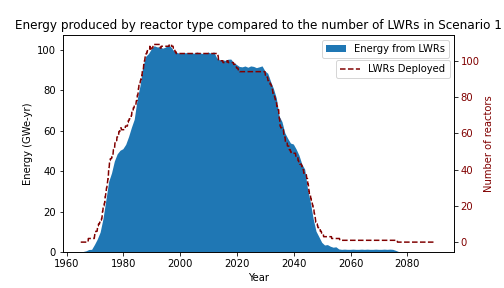
\includegraphics[scale=0.5]{figures/energy_scenario1.png}
    \caption{Energy supplied by \glspl{LWR} compared to the number of 
    \glspl{LWR} deployed in Scenario 1.}
    \label{fig:energy_rx_1}
\end{figure}


\subsection{Scenario 2}

\begin{figure}
    \centering 
    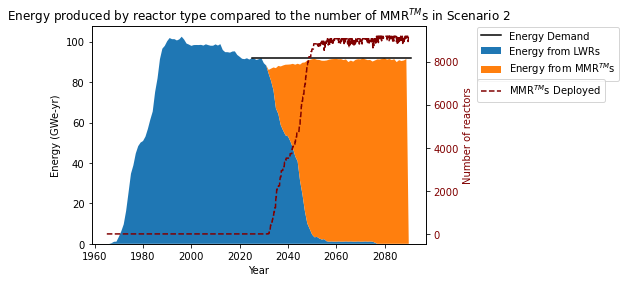
\includegraphics[scale=0.5]{figures/energy_scenario2.png}
    \caption{Energy supplied by each type of reactor compared to the number of 
    \glspl{MMR} deployed in Scenario 2.}
    \label{fig:energy_rx_2}
\end{figure}

\subsection{Scenario 3}

\begin{figure}
    \centering 
    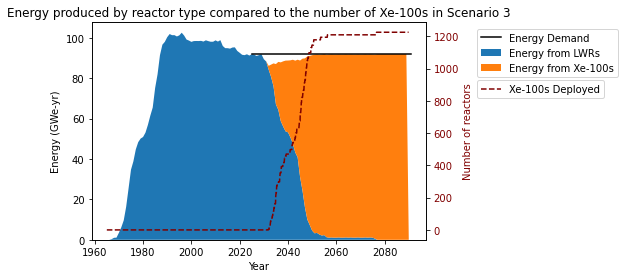
\includegraphics[scale=0.5]{figures/energy_scenario3.png}
    \caption{Energy supplied by each type of reactor compared to the number of 
    Xe-100s deployed in Scenario 3.}
    \label{fig:energy_rx_3}
\end{figure}

\subsection{Scenario 4}

\begin{figure}
    \centering 
    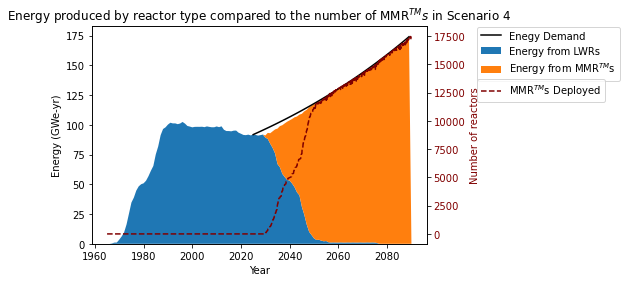
\includegraphics[scale=0.5]{figures/energy_scenario4.png}
    \caption{Energy supplied by each type of reactor compared to the number of 
    \glspl{MMR} deployed in Scenario 4.}
    \label{fig:energy_rx_4}
\end{figure}

\subsection{Scenario 5}

\begin{figure}
    \centering 
    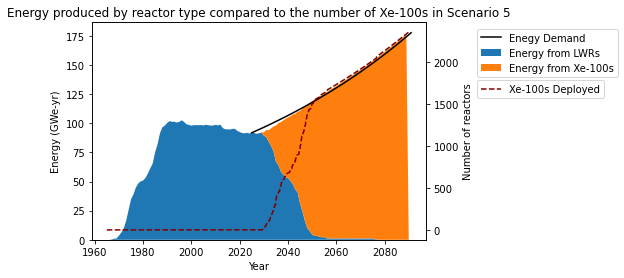
\includegraphics[scale=0.5]{figures/energy_scenario5.png}
    \caption{Energy supplied by each type of reactor compared to the number of 
    Xe-100s deployed in Scenario 5.}
    \label{fig:energy_rx_5}
\end{figure}
